\chapter{Kimia Zat Padat: Pita, Cacat, dan Semikonduktor}\label{ch:b3:solid-state}

Panel surya di atap dan dioda pemancar cahaya di dalam lampu dibuat dari
kristal sejenis, yaitu silikon atau senyawa galium dengan nitrogen, arsenik,
atau fosfor, yang dengan sengaja diberi beberapa atom pengotor per sejuta
atom. Cara kerjanya ditentukan oleh dua hal yang tidak dimiliki molekul: pita
tingkat energi, dengan celah yang lebarnya menetapkan cahaya mana yang diserap
atau dipancarkan kristal, dan cacat, yang membawa muatan. Bab ini membangun
pita dari orbital molekul, menghitung \omterm{def:b3:solid-state:carriers}{pembawa muatan} dalam \omterm{def:b3:solid-state:classes}{semikonduktor}, dan
memperlakukan atom yang hilang dan atom yang salah tempat sebagai spesies
kimia dengan kesetimbangannya sendiri, sampai ke \omterm{def:b3:solid-state:ionic-conductor}{elektrolit padat} sensor
oksigen di saluran buang mobil.

\begin{recall}
Jilid Tahun 1 mendefinisikan kristal, ikatan logam, kristal ionik dan
kristal kovalen, situs interstisial dan paduan, serta persamaan Nernst; Jilid
Tahun 2 mendefinisikan metode Hückel dan integral resonansi $\beta$.
\Cref{ch:b3:x-ray-diffraction} memberikan kisi resiprok dan
\cref{ch:b3:partition-functions} \omterm{def:b3:partition-functions:boltzmann}{distribusi Boltzmann} serta \omterm{def:b3:partition-functions:statistical-entropy}{entropi
statistik} $S = k\ln W$.
\end{recall}

\begin{omfigure}
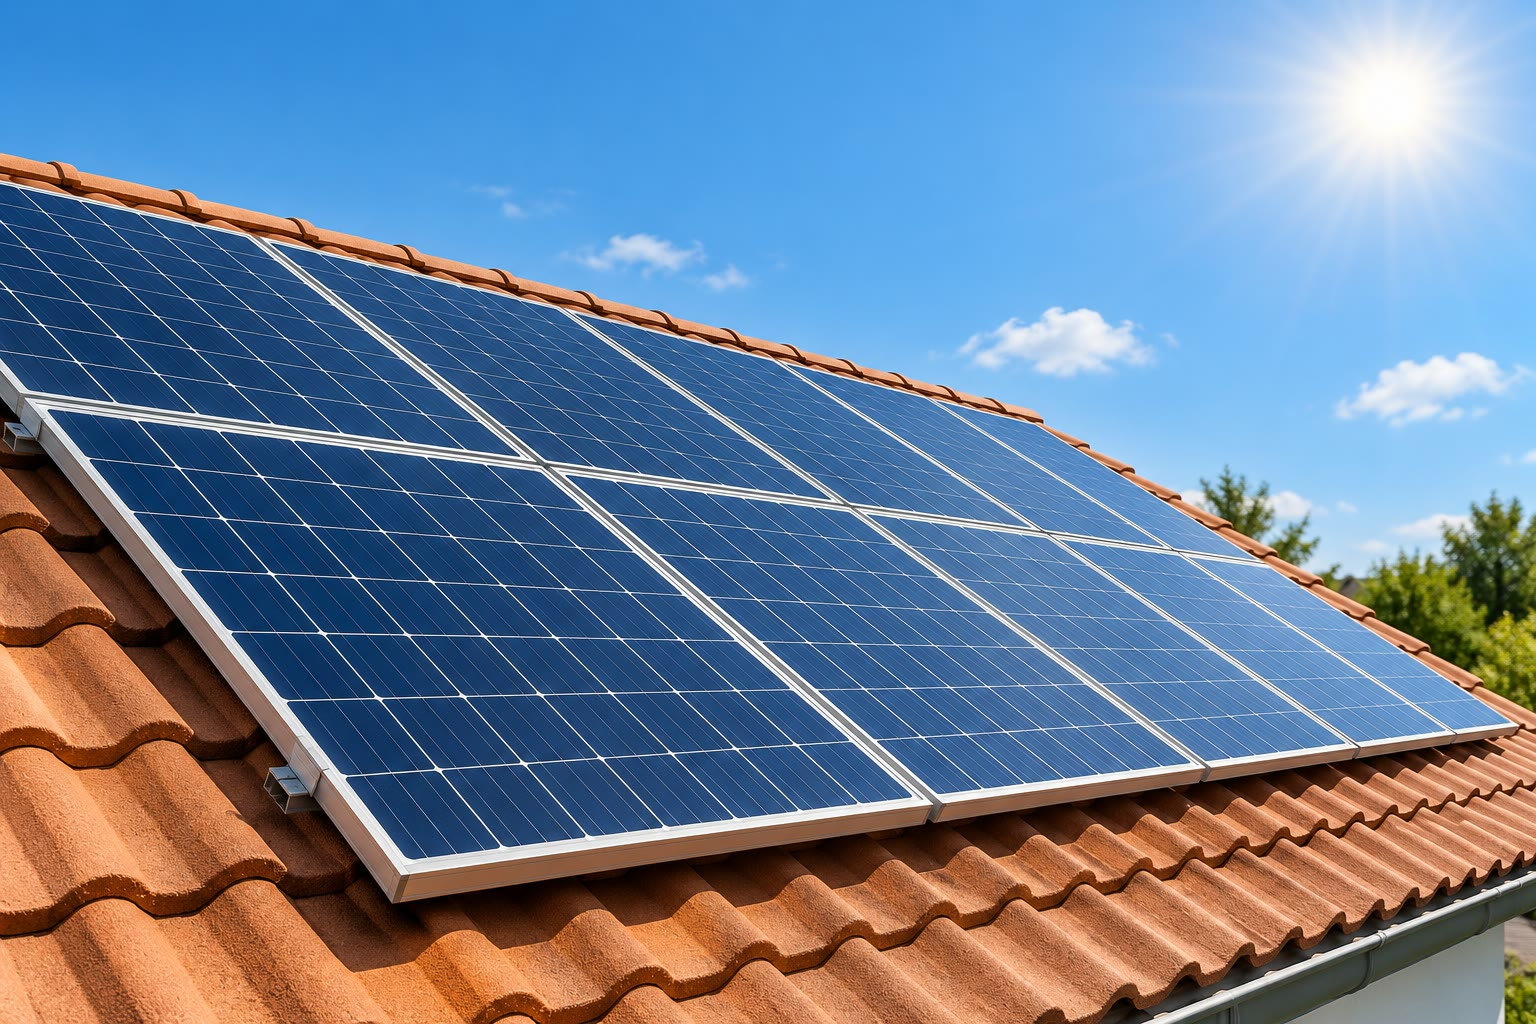
\includegraphics[width=0.6\linewidth]{images/book4/ai/b3-22-solar-panels.jpg}

{\small Panel surya di atap genteng: setiap sel adalah irisan tipis silikon,
tempat cahaya mengangkat elektron melintasi \omterm{def:b3:solid-state:band}{celah pita} sekitar satu elektronvolt.}
\end{omfigure}

\section{Dari orbital ke pita}

Ambillah rantai $N$ atom identik, masing-masing dengan satu orbital s, dalam
pendekatan Hückel: integral Coulomb $\alpha$ pada setiap atom, integral resonansi $\beta < 0$
antara atom-atom yang bertetangga, dan nol untuk pasangan lainnya.

\begin{theorem}[Tingkat-tingkat rantai Hückel]\label{thm:b3:solid-state:chain}
Ke-$N$ orbital molekul rantai linear $N$ atom memiliki energi
\[
  E_k = \alpha + 2\beta\cos\frac{k\pi}{N + 1}, \qquad k = 1, \dots, N,
\]
dengan koefisien $c_j^{(k)} \propto \sin\bigl(jk\pi/(N + 1)\bigr)$ pada atom $j$. Ketika $N \to \infty$, tingkat-tingkat itu mengisi
selang dari $\alpha + 2\beta$ sampai $\alpha - 2\beta$ secara rapat: sebuah pita selebar $4|\beta|$.
\end{theorem}

\begin{proof}
Persamaan sekularnya adalah $\beta c_{j-1} + (\alpha - E)c_j + \beta c_{j+1} = 0$ untuk $j = 1, \dots, N$, dengan $c_0 = c_{N+1} = 0$
(tidak ada atom di sana). Cobalah $c_j = \sin(j\theta)$: karena $\sin((j - 1)\theta) + \sin((j + 1)\theta) = 2\cos\theta\sin(j\theta)$, setiap
persamaan menjadi $(\alpha - E + 2\beta\cos\theta)\sin(j\theta) = 0$, sehingga $E = \alpha + 2\beta\cos\theta$. Syarat $c_0 = 0$ berlaku
untuk setiap $\theta$, dan $c_{N+1} = \sin((N + 1)\theta) = 0$ mensyaratkan $\theta = k\pi/(N + 1)$; $k = 1, \dots, N$ memberikan $N$ tingkat
yang berbeda (nilai-nilai lainnya mengulanginya atau lenyap). Tingkat terendah dan tertinggi adalah
$\alpha \pm 2\beta\cos(\pi/(N + 1))$, yang menuju $\alpha \pm 2\beta$; jarak antara tingkat-tingkat yang bertetangga paling besar
$2|\beta|\pi/(N + 1)$, yang menuju nol.
\end{proof}

Untuk $N = 2$ teorema itu memberikan $\alpha \pm \beta$, yaitu orbital-orbital sistem $\pi$ etena; untuk
$N = 6$, heksatriena rantai terbuka. Dalam tiga dimensi, hal yang sama terjadi pada
setiap jenis orbital atom: orbital s memberikan pita s, orbital p pita p,
dan setiap pita menampung $2N$ elektron untuk $N$ atom.

\begin{definition}[Pita]\label{def:b3:solid-state:band}
Yang disebut \emph{pita energi}\index{pita energi} sebuah kristal adalah rentang kontinu
energi satu-elektron yang diizinkan, yang terbentuk dari orbital-orbital semua atomnya. Yang disebut
\emph{celah pita}\index{celah pita} $E_g$ adalah rentang energi tanpa tingkat di antara dua
pita. Dalam \omterm{def:b3:solid-state:classes}{semikonduktor} atau \omterm{def:b3:solid-state:classes}{isolator} pada suhu nol, pita terisi yang
tertinggi adalah \emph{pita valensi}\index{pita valensi} dan pita kosong yang terendah
adalah \emph{pita konduksi}\index{pita konduksi}.
\end{definition}

\begin{definition}[Rapat keadaan dan tingkat Fermi]\label{def:b3:solid-state:fermi}
Yang disebut \emph{rapat keadaan}\index{rapat keadaan} $g(E)$ adalah jumlah
tingkat per satuan energi (dan per atom atau per satuan volume) di dekat energi $E$.
Yang disebut \emph{tingkat Fermi}\index{tingkat Fermi} $E_F$ adalah energi yang tingkatnya memiliki
peluang $1/2$ untuk terisi; pada suhu nol, semua tingkat di bawahnya
terisi dan semua tingkat di atasnya kosong.
\end{definition}

\begin{omfigure}
\begin{tikzpicture}
\begin{axis}[width=0.78\linewidth, height=6.2cm, xmin=0.3, xmax=7.6, ymin=-2.3, ymax=2.3,
  axis lines=left, xtick={1,2,3,4,5,6.6}, xticklabels={2,4,8,16,64,$\infty$: $g(E)$},
  xlabel={jumlah atom $N$}, ylabel={$(E - \alpha)/|\beta|$},
  ytick={-2,-1,0,1,2}, tick label style={font=\small}, label style={font=\small}]
\addplot[only marks, mark=-, mark size=7pt, omDef, thick] table[x=col, y=e] {figdata/out/bachelor-3-band-chain.dat};
\addplot[omThm, thick] table[x expr=6.0+0.55*\thisrow{g}, y=e] {figdata/out/bachelor-3-band-chain-b.dat};
\draw[black!40, dashed] (axis cs:0.3,-2) -- (axis cs:7.6,-2);
\draw[black!40, dashed] (axis cs:0.3,2) -- (axis cs:7.6,2);
\draw[<->, black!60] (axis cs:5.6,-2) -- (axis cs:5.6,2) node[midway, left, font=\scriptsize] {$4|\beta|$};
\end{axis}
\end{tikzpicture}

{\small Tingkat-tingkat Hückel rantai 2 sampai 64 atom (satu garis pendek per tingkat;
dengan $\beta < 0$ tingkat-tingkat ikatan berada di bawah). Tingkat-tingkat itu memadat menjadi pita
antara $\alpha + 2\beta$ dan $\alpha - 2\beta$; di sebelah kanan, \omterm{def:b3:solid-state:fermi}{rapat keadaan} rantai
tak hingga, yang paling besar di tepi-tepi pita.}
\end{omfigure}

\begin{proposition}[Pengisian pita]\label{prop:b3:solid-state:filling}
Kristal yang pita terisi tertingginya hanya terisi sebagian menghantarkan listrik
seperti logam; kristal yang pita-pitanya terisi penuh atau kosong sama sekali, dengan celah
di antaranya, tidak menghantar pada suhu nol.
\end{proposition}

\begin{proof}[Argumen]
Dalam medan listrik, elektron memperoleh sedikit energi dan momentum: elektron itu harus
berpindah ke tingkat-tingkat kosong tepat di atas tingkat yang ditempatinya. Dalam pita yang
terisi sebagian, tingkat semacam itu terletak tepat di atas \omterm{def:b3:solid-state:fermi}{tingkat Fermi}, tanpa biaya energi. Dalam
pita yang penuh, setiap tingkat sudah terisi dan tingkat kosong berikutnya berada di seberang celah;
lagi pula, pita yang penuh tidak membawa arus neto, karena untuk setiap elektron yang bergerak
ke satu arah ada elektron lain yang bergerak ke arah sebaliknya.
\end{proof}

Natrium, dengan satu elektron 3s per atom, mengisi setengah pita s-nya: sebuah logam.
Magnesium, dengan dua elektron, akan mengisi pita s-nya tepat penuh, tetapi pita s dan pita p
bertumpang tindih, sehingga magnesium juga logam. Intan dan silikon memiliki empat elektron valensi
per atom dalam orbital-orbital yang terpecah menjadi pita ikatan yang terisi dan pita
antiikatan yang kosong, yang dipisahkan oleh sebuah celah.

\begin{definition}[Semikonduktor dan isolator]\label{def:b3:solid-state:classes}
Yang disebut \emph{semikonduktor}\index{semikonduktor} adalah padatan yang \omterm{def:b3:solid-state:band}{celah pitanya} cukup kecil
(sampai sekitar \qty{3}{eV}) sehingga sejumlah elektron yang terukur dapat melintasinya
pada suhu biasa atau setelah didoping; sedangkan \emph{isolator}\index{isolator}
memiliki celah yang begitu besar sehingga tidak menghantar.
\end{definition}

\begin{omfigure}
\begin{tikzpicture}[font=\small]
  \foreach \x/\name in {0/logam, 3.6/semikonduktor, 7.2/isolator} {
    \node[font=\small\bfseries] at (\x+0.8,4.3) {\name};
  }
  % logam: satu pita yang terisi sebagian
  \fill[omDef!55] (0,0.4) rectangle (1.6,2.0);
  \draw (0,0.4) rectangle (1.6,3.4);
  \draw[omThm, thick] (-0.25,2.0) -- (1.85,2.0) node[right, font=\scriptsize] {$E_F$};
  % semikonduktor: celah kecil
  \fill[omDef!55] (3.6,0.4) rectangle (5.2,1.7);
  \draw (3.6,0.4) rectangle (5.2,1.7);
  \draw (3.6,2.5) rectangle (5.2,3.8);
  \draw[omThm, thick] (3.35,2.1) -- (5.45,2.1) node[right, font=\scriptsize] {$E_F$};
  \draw[<->] (4.4,1.7) -- (4.4,2.5) node[pos=0.8, right, font=\scriptsize] {$E_g$};
  % isolator: celah besar
  \fill[omDef!55] (7.2,0.4) rectangle (8.8,1.2);
  \draw (7.2,0.4) rectangle (8.8,1.2);
  \draw (7.2,3.2) rectangle (8.8,4.0);
  \draw[omThm, thick] (6.95,2.2) -- (9.05,2.2) node[right, font=\scriptsize] {$E_F$};
  \draw[<->] (8.0,1.2) -- (8.0,3.2) node[pos=0.75, right, font=\scriptsize] {$E_g$};
  \node[font=\scriptsize, anchor=east] at (3.5,1.05) {valensi};
  \node[font=\scriptsize, anchor=east] at (3.5,3.15) {konduksi};
  \draw[->] (-0.6,0.2) -- (-0.6,3.9) node[above, font=\scriptsize] {$E$};
\end{tikzpicture}

{\small Pengisian pita pada suhu nol (tingkat-tingkat yang terisi diarsir). Logam memiliki
pita yang terisi sebagian dan \omterm{def:b3:solid-state:fermi}{tingkat Fermi} di dalamnya; \omterm{def:b3:solid-state:classes}{semikonduktor} dan
\omterm{def:b3:solid-state:classes}{isolator} memiliki \omterm{def:b3:solid-state:band}{pita valensi} yang penuh dan \omterm{def:b3:solid-state:band}{pita konduksi} yang kosong, dengan \omterm{def:b3:solid-state:fermi}{tingkat
Fermi} di dalam celah, yang sempit pada \omterm{def:b3:solid-state:classes}{semikonduktor} dan lebar pada \omterm{def:b3:solid-state:classes}{isolator}.}
\end{omfigure}

\section{Semikonduktor}

\begin{definition}[Pembawa muatan]\label{def:b3:solid-state:carriers}
Yang disebut \emph{semikonduktor intrinsik}\index{semikonduktor intrinsik} adalah \omterm{def:b3:solid-state:classes}{semikonduktor}
murni, yang semua pembawa muatannya berasal dari elektron yang tereksitasi melintasi celah. Yang disebut
\emph{pembawa muatan}\index{pembawa muatan} adalah partikel bergerak yang membawa
arus: elektron di \omterm{def:b3:solid-state:band}{pita konduksi}, atau \emph{lubang}\index{lubang}, yaitu
tingkat kosong di \omterm{def:b3:solid-state:band}{pita valensi}, yang bergerak seperti muatan positif.
\end{definition}

\begin{theorem}[Konsentrasi pembawa intrinsik]\label{thm:b3:solid-state:intrinsic}
Dengan $N_c$ dan $N_v$ \omterm{def:b3:solid-state:fermi}{rapat keadaan} efektif \omterm{def:b3:solid-state:band}{pita konduksi} dan \omterm{def:b3:solid-state:band}{pita
valensi} (diterima tanpa bukti), konsentrasi elektron dan \omterm{def:b3:solid-state:carriers}{lubang} sebuah \omterm{def:b3:solid-state:classes}{semikonduktor}
yang \omterm{def:b3:solid-state:fermi}{tingkat Fermi-nya} berjarak lebih dari beberapa $kT$ dari kedua tepi pita adalah
\[
  n = N_c\,\eu^{-(E_c - E_F)/kT}, \qquad p = N_v\,\eu^{-(E_F - E_v)/kT},
\]
dan dalam \omterm{def:b3:solid-state:carriers}{semikonduktor intrinsik}
\[
  n = p = n_i = \sqrt{N_cN_v}\,\eu^{-E_g/2kT}.
\]
\end{theorem}

\begin{proof}
Okupansi tingkat berenergi $E$ adalah $f(E) = 1/(1 + \eu^{(E - E_F)/kT})$. Jika
$E - E_F \gg kT$, $f \approx \eu^{-(E - E_F)/kT}$, yaitu ekor Boltzmann. Dengan menjumlahkannya atas tingkat-tingkat \omterm{def:b3:solid-state:band}{pita
konduksi}, $n = \int g_c(E)\eu^{-(E - E_F)/kT}\,\dd E = \eu^{-(E_c - E_F)/kT}\int g_c(E)\eu^{-(E - E_c)/kT}\,\dd E$, dan integral terakhir itu menurut
definisi adalah $N_c$. \omterm{def:b3:solid-state:carriers}{Lubang} adalah tingkat kosong, dengan peluang $1 - f \approx \eu^{-(E_F - E)/kT}$ di
\omterm{def:b3:solid-state:band}{pita valensi}; langkah-langkah yang sama memberikan $p$. Maka $np = N_cN_v\eu^{-(E_c - E_v)/kT} = N_cN_v\eu^{-E_g/kT}$, dan dalam kristal murni
setiap elektron yang tereksitasi meninggalkan satu \omterm{def:b3:solid-state:carriers}{lubang}: $n = p$, sehingga $n = \sqrt{np}$.
\end{proof}

\begin{proposition}[Hukum aksi massa]\label{prop:b3:solid-state:mass-action}
Dalam setiap \omterm{def:b3:solid-state:classes}{semikonduktor} pada kesetimbangan, didoping atau tidak, $np = n_i^2$.
\end{proposition}

\begin{proof}
Hasil kali $np = N_cN_v\eu^{-E_g/kT}$ yang diperoleh dalam bukti
\cref{thm:b3:solid-state:intrinsic} tidak mengandung $E_F$: nilainya sama apa pun yang
menetapkan \omterm{def:b3:solid-state:fermi}{tingkat Fermi}, dan sama dengan nilai intrinsiknya $n_i^2$. Hasil kali itu adalah
tetapan kesetimbangan $\text{nihil} \rightleftharpoons \mathrm e^- + \mathrm h^+$, seperti hasil kali ion air.
\end{proof}

\begin{omfigure}
% ledger: eg:Si.E0, eg:Si.a, eg:Si.b, eg:Ge.E0, eg:Ge.a, eg:Ge.b, dos:Si.Nc, dos:Si.Nv, dos:Ge.Nc, dos:Ge.Nv, dop:Si.P
\begin{tikzpicture}
\begin{axis}[name=a, width=0.45\linewidth, height=5.6cm, xmin=1.2, xmax=4.2, ymin=4, ymax=18,
  axis lines=left, xlabel={$1000\,\mathrm K/T$}, ylabel={$\log_{10}(n_i/\unit{cm^{-3}})$},
  tick label style={font=\scriptsize}, label style={font=\small}]
\addplot[omDef, thick] table[x=invT, y=lgSi] {figdata/out/bachelor-3-semiconductor-carriers.dat};
\addplot[omThm, thick] table[x=invT, y=lgGe] {figdata/out/bachelor-3-semiconductor-carriers.dat};
\node[font=\scriptsize, omDef] at (axis cs:3.4,8.3) {Si};
\node[font=\scriptsize, omThm, anchor=south west] at (axis cs:3.4,14.0) {Ge};
\end{axis}
\begin{axis}[at={(a.east)}, anchor=west, xshift=1.7cm, width=0.45\linewidth, height=5.6cm,
  xmin=1, xmax=25, ymin=10, ymax=17, axis lines=left,
  xlabel={$1000\,\mathrm K/T$}, ylabel={$\log_{10}(n/\unit{cm^{-3}})$},
  tick label style={font=\scriptsize}, label style={font=\small}]
\addplot[omDef, thick] table[x=invT, y=lgn] {figdata/out/bachelor-3-semiconductor-carriers-b.dat};
\addplot[black!45, dashed, unbounded coords=jump, restrict y to domain=10:17] table[x=invT, y=lgni] {figdata/out/bachelor-3-semiconductor-carriers-b.dat};
\node[font=\scriptsize, anchor=west] at (axis cs:2.6,16.4) {intrinsik};
\node[font=\scriptsize] at (axis cs:12,15.35) {saturasi, $n = N_D$};
\node[font=\scriptsize] at (axis cs:20,13.2) {pembekuan};
\end{axis}
\end{tikzpicture}

{\small Kiri: konsentrasi pembawa intrinsik silikon dan germanium terhadap
$1/T$ (model dengan celah dan \omterm{def:b3:solid-state:fermi}{rapat keadaan} efektif yang terukur); kemiringannya
mendekati $-E_g/2k$. Kanan: elektron dalam silikon yang didoping
$\qty{1e15}{cm^{-3}}$ fosfor: pada suhu rendah, donor-donor menahan elektronnya
(pembekuan), dari sekitar 150 sampai \qty{500}{K} semuanya terionisasi ($n = N_D$), dan pada suhu
tinggi pembawa intrinsik (putus-putus, $n_i$) mengambil alih.}
\end{omfigure}

\begin{definition}[Celah langsung dan tak langsung]\label{def:b3:solid-state:gap-types}
Sebuah \omterm{def:b3:solid-state:classes}{semikonduktor} memiliki \emph{celah pita langsung}\index{celah pita langsung} jika
puncak \omterm{def:b3:solid-state:band}{pita valensinya} dan dasar \omterm{def:b3:solid-state:band}{pita konduksinya} terjadi pada momentum elektron yang
sama, sehingga sebuah foton saja dapat membawa elektron melintasinya, dan memiliki
\emph{celah pita tak langsung}\index{celah pita tak langsung} jika tidak demikian, sehingga
transisinya juga memerlukan sebuah vibrasi kisi.
\end{definition}

% ledger: eg:Si, eg:Ge, eg:GaAs, eg:GaN, eg:GaP
Silikon (\qty{1.12}{eV}) dan germanium (\qty{0.66}{eV}) memiliki celah tak langsung:
keduanya menyerap cahaya cukup baik dalam lapisan yang tebal, yang cocok untuk sel surya, tetapi
memancarkannya dengan sangat buruk. Galium arsenida (\qty{1.42}{eV}) dan galium nitrida (sekitar
\qty{3.4}{eV}) memiliki celah langsung, yang menjadi dasar dioda pemancar cahaya inframerah dan biru
serta laser; galium fosfida (\qty{2.26}{eV}) bercelah tak langsung tetapi memancarkan cahaya hijau
jika didoping. Warna banyak pigmen juga merupakan \omterm{def:b3:solid-state:band}{celah pita}: sebuah kristal
menyerap semua foton dengan $h\nu > E_g$, sehingga kadmium sulfida, yang celahnya berada di daerah biru,
berwarna kuning.

\begin{definition}[Doping]\label{def:b3:solid-state:doping}
Yang disebut \emph{dopan}\index{dopan} adalah atom asing yang dengan sengaja dimasukkan ke dalam \omterm{def:b3:solid-state:classes}{semikonduktor},
dalam jumlah kecil, untuk menyediakan \omterm{def:b3:solid-state:carriers}{pembawa muatan}. Dalam \emph{semikonduktor
tipe-n}\index{semikonduktor tipe-n}, dopan memiliki satu elektron valensi lebih banyak
daripada atom yang digantikannya (fosfor dalam silikon) dan memberikannya ke
\omterm{def:b3:solid-state:band}{pita konduksi} dari \emph{tingkat donor}\index{tingkat donor} tepat di bawah pita
itu; dalam \emph{semikonduktor tipe-p}\index{semikonduktor tipe-p}, dopan memiliki satu elektron
lebih sedikit (boron dalam silikon) dan menerima elektron dari \omterm{def:b3:solid-state:band}{pita valensi} ke dalam
\emph{tingkat akseptor}\index{tingkat akseptor} tepat di atasnya, sehingga tertinggal sebuah \omterm{def:b3:solid-state:carriers}{lubang}.
\end{definition}

\begin{omfigure}
\begin{tikzpicture}[font=\small]
  \foreach \x in {0, 5.2} {
    \fill[omDef!35] (\x,0) rectangle (\x+3.6,1.0);
    \fill[omDef!12] (\x,2.6) rectangle (\x+3.6,3.6);
    \node[font=\scriptsize] at (\x+1.8,0.5) {pita valensi};
    \node[font=\scriptsize] at (\x+1.8,3.1) {pita konduksi};
  }
  \foreach \i in {0,...,5} { \draw[omThm, thick] (0.25+\i*0.55,2.35) -- (0.6+\i*0.55,2.35); }
  \node[font=\scriptsize, anchor=west] at (0.1,1.95) {tingkat donor, \qty{0.045}{eV} di bawah};
  \draw[->, omThm] (0.42,2.42) -- (0.42,2.9);
  \fill[omThm] (0.42,2.95) circle (1.6pt);
  \foreach \i in {0,...,5} { \draw[omMeth, thick] (5.45+\i*0.55,1.25) -- (5.8+\i*0.55,1.25); }
  \node[font=\scriptsize, anchor=west] at (5.3,1.6) {tingkat akseptor, \qty{0.045}{eV} di atas};
  \draw[->, omMeth] (5.62,0.7) -- (5.62,1.18);
  \draw[omMeth, fill=white] (5.62,0.62) circle (1.8pt);
  \node[font=\small\bfseries] at (1.8,4.0) {tipe-n: P dalam Si};
  \node[font=\small\bfseries] at (7.0,4.0) {tipe-p: B dalam Si};
\end{tikzpicture}

{\small \omterm{def:b3:solid-state:doping}{Tingkat donor} dan \omterm{def:b3:solid-state:doping}{tingkat akseptor} di dalam celah silikon (celahnya tidak berskala:
tingkat-tingkat \omterm{def:b3:solid-state:doping}{dopan} terletak sekitar 0.045 eV dari tepi pita, sedangkan celahnya 1.12 eV).
Donor memberikan elektronnya (titik) ke \omterm{def:b3:solid-state:band}{pita konduksi}; akseptor mengambil satu elektron
dari \omterm{def:b3:solid-state:band}{pita valensi}, sehingga tertinggal sebuah \omterm{def:b3:solid-state:carriers}{lubang} (lingkaran).}
\end{omfigure}

% ledger: dop:Si.P, dop:Si.B
\omterm{def:b3:solid-state:doping}{Tingkat donor} fosfor terletak \qty{0.045}{eV} di bawah \omterm{def:b3:solid-state:band}{pita konduksi}
silikon, kurang dari $2kT$ pada suhu kamar, dan \omterm{def:b3:solid-state:doping}{tingkat akseptor} boron sama jauhnya
di atas \omterm{def:b3:solid-state:band}{pita valensi}: pada \qty{300}{K} hampir setiap \omterm{def:b3:solid-state:doping}{dopan} terionisasi. Itulah sebabnya
satu atom \omterm{def:b3:solid-state:doping}{dopan} per $10^7$ atom silikon ($\qty{5e15}{cm^{-3}}$) menaikkan
konsentrasi elektron beberapa ratus ribu kali.

\begin{method}[Pembawa muatan semikonduktor yang didoping]\label{met:b3:solid-state:doping}
\begin{enumerate}
  \item Periksalah bahwa suhunya berada dalam rentang saturasi (\omterm{def:b3:solid-state:doping}{dopan} terionisasi
        sepenuhnya, $N_D \gg n_i$): maka pembawa mayoritasnya $n \approx N_D$ (atau $p \approx N_A$).
  \item Peroleh pembawa minoritas dari hukum aksi massa: $p = n_i^2/N_D$.
  \item Tempatkan \omterm{def:b3:solid-state:fermi}{tingkat Fermi}: $E_c - E_F = kT\ln(N_c/n)$, atau relatif terhadap tingkat intrinsik,
        $E_F - E_i = kT\ln(n/n_i)$.
  \item Jika kedua jenis \omterm{def:b3:solid-state:doping}{dopan} hadir, pakailah selisih $N_D - N_A$.
\end{enumerate}
\end{method}

\begin{definition}[Sambungan p--n]\label{def:b3:solid-state:junction}
Yang disebut \emph{sambungan p--n}\index{sambungan p--n} adalah batas, di dalam satu kristal,
antara daerah tipe-p dan daerah tipe-n.
\end{definition}

Pada \omterm{def:b3:solid-state:junction}{sambungan p--n}, elektron berdifusi dari sisi n ke sisi p dan \omterm{def:b3:solid-state:carriers}{lubang}
ke arah sebaliknya, sehingga tertinggal lapisan tipis yang kosong dari \omterm{def:b3:solid-state:carriers}{pembawa muatan}, tempat
\omterm{def:b3:solid-state:doping}{dopan-dopan} terionisasi yang tetap membangkitkan medan listrik; pada kesetimbangan, \omterm{def:b3:solid-state:fermi}{tingkat Fermi}
sama di kedua sisi. Tegangan yang diberikan ke satu arah menurunkan penghalang dan arus
mengalir; ke arah lain tegangan itu menaikkannya: sebuah dioda. Dalam dioda pemancar cahaya, elektron
dan \omterm{def:b3:solid-state:carriers}{lubang} yang diinjeksikan melintasi sambungan bergabung kembali dan memancarkan foton dengan energi
yang mendekati $E_g$; dalam sel surya, foton yang diserap di dekat sambungan menghasilkan
pasangan elektron--lubang yang dipisahkan oleh medan, dan arus mengalir dalam
rangkaian luar.

\begin{omfigure}
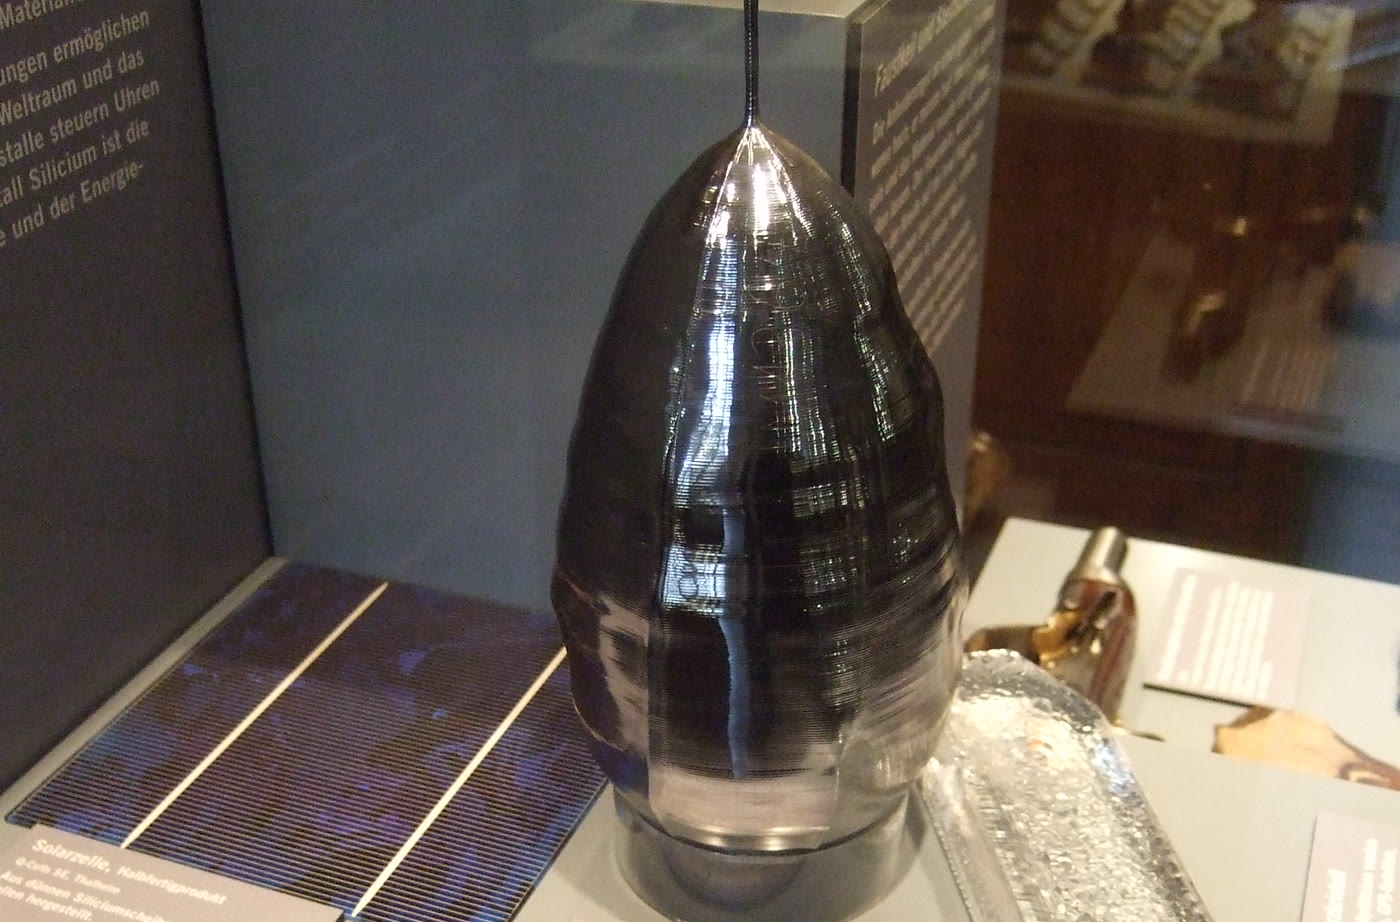
\includegraphics[width=0.5\linewidth]{images/book4/silicon-boule.jpg}

{\small Kristal tunggal silikon yang ditarik dari lelehan, diperlihatkan di samping sel
surya yang dibuat dari irisan kristal semacam itu. Foto: Sebastian Wallroth,
domain publik.}
\end{omfigure}

\begin{inthelab}[Menumbuhkan kristal silikon]
Dalam metode Czochralski, silikon polikristalin yang sangat murni dilelehkan dalam
krus silika di bawah argon, sedikit di atas titik lelehnya, dengan
\omterm{def:b3:solid-state:doping}{dopan} yang ditambahkan ke dalam lelehan. Sebuah kristal benih kecil pada batang yang berputar dicelupkan ke dalam
lelehan dan perlahan-lahan diangkat: silikon mengkristal padanya dengan orientasi
benih itu, dan laju penarikan serta putaran menetapkan diameternya. Bola kristal
itu kemudian digergaji menjadi wafer yang tebalnya kurang dari satu milimeter. Silana dan gas-gas
doping fosfina dan arsina yang dipakai pada tahap-tahap selanjutnya bersifat piroforik atau sangat beracun,
dan hanya ditangani dalam sistem industri yang tertutup rapat.
\end{inthelab}

\section{Cacat titik}

\begin{definition}[Cacat titik]\label{def:b3:solid-state:defects}
Yang disebut \emph{cacat titik}\index{cacat titik} adalah penyimpangan dari kristal sempurna
yang terlokalisasi pada satu situs: kekosongan, atom interstisial, atau atom
asing. Dalam kristal ionik, yang disebut \emph{cacat Schottky}\index{cacat Schottky} adalah
sepasang kekosongan, satu kation dan satu anion, yang ion-ionnya telah pindah ke
permukaan; sedangkan \emph{cacat Frenkel}\index{cacat Frenkel} adalah pasangan yang terdiri atas
sebuah kekosongan dan ion yang meninggalkannya, yang kini menempati situs interstisial.
\end{definition}

\begin{omfigure}
\begin{tikzpicture}[scale=0.62]
  \begin{scope}
  \foreach \i in {0,...,5} \foreach \j in {0,...,4} {
    \pgfmathtruncatemacro{\pty}{mod(\i+\j,2)}
    \ifnum\pty=0 \fill[omDef!70] (\i,\j) circle (0.2); \else \fill[omThm!25] (\i,\j) circle (0.38); \draw[omThm!60] (\i,\j) circle (0.38); \fi
  }
  \fill[white] (2,2) circle (0.45); \draw[dashed] (2,2) circle (0.3);
  \fill[white] (3,2) circle (0.45); \draw[dashed] (3,2) circle (0.38);
  \node[font=\small\bfseries] at (2.5,5.0) {Schottky (NaCl)};
  \end{scope}
  \begin{scope}[xshift=8cm]
  \foreach \i in {0,...,5} \foreach \j in {0,...,4} {
    \pgfmathtruncatemacro{\pty}{mod(\i+\j,2)}
    \ifnum\pty=0 \fill[black!45] (\i,\j) circle (0.2); \else \fill[omMeth!25] (\i,\j) circle (0.38); \draw[omMeth!60] (\i,\j) circle (0.38); \fi
  }
  \fill[white] (2,2) circle (0.3); \draw[dashed] (2,2) circle (0.22);
  \fill[black!45] (2.5,2.5) circle (0.2);
  \draw[->, thick] (2.1,2.1) -- (2.38,2.38);
  \node[font=\small\bfseries] at (2.5,5.0) {Frenkel (AgCl)};
  \end{scope}
\end{tikzpicture}

{\small \omterm{def:b3:solid-state:defects}{Cacat titik} dalam satu lapisan kristal garam batu (titik kecil: kation;
lingkaran besar: anion; putus-putus: kekosongan). Kiri: pasangan Schottky, yaitu satu kation
dan satu anion yang hilang. Kanan: pasangan Frenkel, yaitu ion perak yang berpindah dari situsnya
ke posisi interstisial.}
\end{omfigure}

\begin{theorem}[Konsentrasi kesetimbangan cacat Schottky]\label{thm:b3:solid-state:schottky}
Dalam kristal MX dengan $N$ satuan rumus, jumlah $n$ pasangan Schottky pada
kesetimbangan, dengan entalpi pembentukan $\Delta H_S$ per pasangan dan $n \ll N$, adalah
\[
  \frac{n}{N} = \eu^{-\Delta H_S/2kT}.
\]
\end{theorem}

\begin{proof}
Pembentukan $n$ pasangan memerlukan $n\,\Delta H_S$ dan memberikan entropi konfigurasi, dari
$\binom{N}{n}$ cara memilih kekosongan kation dan sebanyak itu pula untuk anion:
$S = 2k\ln\frac{N!}{n!(N - n)!}$. Dengan rumus Stirling $\ln x! \approx x\ln x - x$,
\[
  G(n) = n\,\Delta H_S - 2kT\bigl[N\ln N - n\ln n - (N - n)\ln(N - n)\bigr].
\]
Pada kesetimbangan $\dd G/\dd n = 0$: $\Delta H_S - 2kT\ln\frac{N - n}{n} = 0$, sehingga $n/(N - n) = \eu^{-\Delta H_S/2kT}$, dan $n/N$ untuk
$n \ll N$. Entropi vibrasi cacat-cacat itu, yang diabaikan di sini, mengalikan
hasilnya dengan sebuah faktor tetap.
\end{proof}

\begin{proposition}[Cacat Frenkel]\label{prop:b3:solid-state:frenkel}
Dengan $N$ ion dari jenis yang berpindah, $N_i$ situs interstisial yang tersedia baginya, dan
$\Delta H_F$ entalpi pembentukan sebuah pasangan, jumlah pasangan Frenkel adalah $n =
\sqrt{NN_i}\,\eu^{-\Delta H_F/2kT}$ (untuk $n \ll N, N_i$).
\end{proposition}

\begin{proof}
Entropinya kini $S = k\ln\binom{N}{n} + k\ln\binom{N_i}{n}$, dan minimisasi yang sama memberikan
\[
  \Delta H_F = kT\ln\frac{(N - n)(N_i - n)}{n^2} \approx kT\ln\frac{NN_i}{n^2},
\]
dan dari situ hasilnya.
\end{proof}

Akar kuadrat itu menunjukkan bahwa cacat terbentuk berpasangan: seperti $n_i$ dalam \omterm{def:b3:solid-state:classes}{semikonduktor},
konsentrasinya memiliki setengah energi pembentukan dalam eksponennya. Halida alkali
terutama membentuk \omterm{def:b3:solid-state:defects}{cacat Schottky}; halida perak, yang ion
$\ce{Ag+}$-nya kecil dan mudah terpolarisasi sehingga muat di antara anion-anion, terutama membentuk \omterm{def:b3:solid-state:defects}{cacat Frenkel}.

\begin{definition}[Notasi Kröger--Vink]\label{def:b3:solid-state:kroger-vink}
Yang disebut \emph{notasi Kröger--Vink}\index{notasi Kröger--Vink} adalah notasi yang menuliskan \omterm{def:b3:solid-state:defects}{cacat titik}
sebagai $\mathrm{A_S^c}$: A adalah spesies pada situs itu (V untuk kekosongan, $i$ sebagai situs
untuk interstisial), S situs yang ditempatinya dalam kristal sempurna, dan c muatannya
relatif terhadap situs itu: $\bullet$ untuk setiap satuan positif, $'$ untuk setiap satuan
negatif, $\times$ jika tidak ada.
\end{definition}

Jadi $\mathrm{V_{Na}'}$ adalah kekosongan natrium ($+1$ yang hilang meninggalkan muatan relatif $-1$),
$\mathrm{V_{Cl}^{\bullet}}$ kekosongan klorida, $\mathrm{Ag_i^{\bullet}}$ ion perak interstisial, $\mathrm{Ca_{Na}^{\bullet}}$ ion kalsium pada
situs natrium, $\mathrm{O_O^{\times}}$ ion oksida pada tempatnya. Kesetimbangan Schottky NaCl adalah
$\text{nihil} \rightleftharpoons \mathrm{V_{Na}' + V_{Cl}^{\bullet}}$, sedangkan kesetimbangan Frenkel AgCl adalah
$\mathrm{Ag_{Ag}^{\times}} \rightleftharpoons \mathrm{Ag_i^{\bullet} + V_{Ag}'}$.

\begin{method}[Menuliskan persamaan cacat]\label{met:b3:solid-state:kroger-vink}
\begin{enumerate}
  \item Tuliskan apa yang ditambahkan ke kristal induk dan cacat-cacat yang ditimbulkannya.
  \item Neraca situs: rasio situs kation terhadap situs anion kristal induk dipertahankan
        (kekosongan dihitung sebagai situs).
  \item Neraca massa: atom-atom yang sama di kedua sisi (kekosongan tidak bermassa;
        elektron $e'$ dan \omterm{def:b3:solid-state:carriers}{lubang} $h^\bullet$ juga tidak).
  \item Neraca muatan: jumlah muatan efektifnya sama.
\end{enumerate}
\end{method}

\begin{example}[Itria dalam zirkonia]
Melarutkan $\ce{Y2O3}$ dalam $\ce{ZrO2}$ menempatkan dua $\ce{Y^3+}$ pada situs $\ce{Zr^4+}$, masing-masing bermuatan relatif $-1$, dan
tiga ion oksida pada situs oksigen; rasio satu kation terhadap dua situs oksigen kristal induk
mensyaratkan empat situs oksigen untuk kedua kation, sehingga satu situs tetap kosong:
\[
  \ce{Y2O3} \xrightarrow{\ce{ZrO2}} \mathrm{2\,Y_{Zr}' + 3\,O_O^{\times} + V_O^{\bullet\bullet}}.
\]
Situs: 2 kation, 4 oksigen; massa: 2 Y dan 3 O; muatan: $2(-1) + 2 = 0$. Satu kekosongan
oksida untuk setiap dua ion itrium: inilah yang membuat zirkonia yang distabilkan itria
menjadi konduktor ion oksida.
\end{example}

\begin{definition}[Pusat warna]\label{def:b3:solid-state:colour-centre}
Yang disebut \emph{pusat warna}\index{pusat warna} adalah \omterm{def:b3:solid-state:defects}{cacat titik} yang menyerap
cahaya tampak, misalnya elektron yang terperangkap dalam kekosongan anion sebuah halida
alkali (pusat F), yang mewarnai kristal yang sebenarnya transparan.
\end{definition}

Memanaskan natrium klorida dalam uap natrium atau menyinarinya menghasilkan pusat F:
elektron yang terperangkap berperilaku seperti \omterm{def:b3:quantum-model-systems:box}{partikel dalam kotak} seukuran kekosongan itu, dan
menyerap di daerah tampak, sehingga kristalnya menjadi kuning kecokelatan.

\section{Nonstoikiometri}

\begin{definition}[Senyawa nonstoikiometrik]\label{def:b3:solid-state:non-stoichiometric}
Yang disebut \emph{senyawa nonstoikiometrik}\index{senyawa nonstoikiometrik} adalah
padatan yang komposisinya bervariasi dalam suatu rentang di sekitar perbandingan sederhana bilangan
bulat, dengan selisihnya ditampung oleh \omterm{def:b3:solid-state:defects}{cacat titik}.
\end{definition}

Besi(II) oksida tidak pernah tepat $\ce{FeO}$: senyawa itu selalu kekurangan besi,
$\mathrm{Fe_{1-x}O}$, dengan $x$ yang ditentukan oleh suhu dan tekanan oksigen saat senyawa itu dibuat. Setiap $\ce{Fe^2+}$ yang hilang diimbangi oleh dua
$\ce{Fe^3+}$, yang dalam bahasa cacat merupakan \omterm{def:b3:solid-state:carriers}{lubang} pada situs besi.

\begin{proposition}[Konduktivitas dan tekanan oksigen]\label{prop:b3:solid-state:brouwer}
Untuk oksida yang kekurangan logam $\mathrm{M_{1-x}O}$ yang cacat-cacatnya berupa kekosongan logam bermuatan ganda
yang diimbangi oleh \omterm{def:b3:solid-state:carriers}{lubang}, konsentrasi \omterm{def:b3:solid-state:carriers}{lubang}, dan konduktivitasnya, berubah sebanding dengan
$p(\ce{O2})^{1/6}$. Untuk oksida yang kekurangan oksigen dan diimbangi oleh elektron, keduanya berubah sebanding dengan
$p(\ce{O2})^{-1/6}$.
\end{proposition}

\begin{proof}
Pengambilan oksigen menciptakan kekosongan logam:
\[
  \tfrac12\ce{O2} \rightleftharpoons \mathrm{O_O^{\times} + V_M'' + 2\,h^{\bullet}}, \qquad K = \frac{[\mathrm{V_M''}][\mathrm h^\bullet]^2}{p(\ce{O2})^{1/2}}
\]
(aktivitas $\mathrm{O_O^{\times}}$ adalah 1). Neraca
muatannya adalah $[\mathrm h^\bullet] = 2[\mathrm{V_M''}]$, sehingga $[\mathrm h^\bullet]^3 = 2K\,p(\ce{O2})^{1/2}$ dan $[\mathrm h^\bullet] \propto p(\ce{O2})^{1/6}$. Untuk
kasus kekurangan oksigen, $\mathrm{O_O^{\times}} \rightleftharpoons \tfrac12\ce{O2} + \mathrm{V_O^{\bullet\bullet} + 2\,e'}$, $[\mathrm e'] = 2[\mathrm{V_O^{\bullet\bullet}}]$, dan langkah-langkah yang sama memberikan $[\mathrm e'] \propto p(\ce{O2})^{-1/6}$.
Konduktivitasnya sebanding dengan konsentrasi \omterm{def:b3:solid-state:carriers}{pembawa muatan}.
\end{proof}

Jadi alur $\log\sigma$ terhadap $\log p(\ce{O2})$ menunjukkan cacat mana yang dominan: kemiringannya,
$\pm 1/4$ atau $\pm 1/6$, bergantung pada muatannya.

\section{Konduktor ionik}

\begin{definition}[Konduktor ionik]\label{def:b3:solid-state:ionic-conductor}
Yang disebut \emph{konduktor ionik}\index{konduktor ionik} adalah padatan yang arusnya
dibawa oleh ion-ion yang bergerak melalui kisi. Yang disebut \emph{elektrolit
padat}\index{elektrolit padat} adalah konduktor ionik yang konduktivitas elektroniknya
dapat diabaikan, sehingga dapat memisahkan kedua elektrode sebuah
sel elektrokimia.
\end{definition}

\begin{proposition}[Hukum Arrhenius konduksi ionik]\label{prop:b3:solid-state:ionic-arrhenius}
Untuk ion-ion yang bergerak dengan melompat di antara situs-situs yang bertetangga melewati penghalang $E_a$,
$\sigma T = A\,\eu^{-E_a/kT}$.
\end{proposition}

\begin{proof}[Bukti parsial]
Sebuah ion mencoba melompat dengan frekuensi $\nu_0$ dan berhasil dengan peluang $\eu^{-E_a/kT}$,
sehingga koefisien difusinya adalah $D = \tfrac16\nu_0 z a^2\eu^{-E_a/kT}$ untuk $z$ situs tetangga pada
jarak $a$ (jalan acak). Hubungan Nernst--Einstein $\sigma = nq^2D/kT$ (diterima tanpa bukti), untuk $n$
ion bergerak bermuatan $q$ per satuan volume, memberikan $\sigma T = (nq^2\nu_0za^2/6k)\,\eu^{-E_a/kT}$.
Konsentrasi $n$ ditetapkan oleh doping dalam konduktor ekstrinsik; jika konsentrasi itu
sendiri terbentuk secara termal, $E_a$ juga memuat setengah entalpi pembentukannya.
\end{proof}

% ledger: trans:AgI
Tiga \omterm{def:b3:solid-state:ionic-conductor}{elektrolit padat} memperlihatkan rentangnya. Dalam zirkonia yang distabilkan itria,
kekosongan oksida yang dihasilkan \omterm{def:b3:solid-state:doping}{dopan} memungkinkan ion $\ce{O^2-}$ melompat; zirkonia itu menghantar dengan baik
hanya jika panas, pada beberapa ratus derajat Celsius. Dalam alumina-$\beta$, ion-ion natrium bergerak di
bidang-bidang yang tersusun longgar di antara blok-blok spinel, yang menjadi dasar baterai
natrium--belerang. Perak iodida menjadi konduktor superionik di atas \qty{146}{\celsius},
tempat ion-ion peraknya tersebar pada situs yang jauh lebih banyak daripada jumlah ionnya,
hampir seperti cairan di dalam kisi iodida yang kaku. Konduktor ion litium
(garnet litium lantanum zirkonat, sulfida) adalah elektrolit baterai
padat sepenuhnya yang kini sedang dikembangkan.

\begin{omfigure}
\begin{tikzpicture}[font=\small, >=Stealth]
  \fill[omProp!25] (0,0) rectangle (2.4,3.2);
  \node[font=\scriptsize, align=center] at (1.2,0.6) {$\ce{ZrO2}$--$\ce{Y2O3}$\\ elektrolit padat};
  \draw[black!60, line width=2.5pt] (-0.07,0) -- (-0.07,3.2);
  \draw[black!60, line width=2.5pt] (2.47,0) -- (2.47,3.2);
  \node[font=\scriptsize, align=center] at (-2.0,1.4) {gas buang\\ $p(\ce{O2})$ rendah};
  \node[font=\scriptsize, align=center] at (4.4,1.4) {udara acuan\\ $p(\ce{O2}) = \qty{0.21}{bar}$};
  \node[font=\scriptsize, anchor=north] at (-0.07,-0.05) {Pt};
  \node[font=\scriptsize, anchor=north] at (2.47,-0.05) {Pt};
  \draw[->, thick, omThm] (2.0,1.9) -- (0.4,1.9) node[midway, above, font=\scriptsize] {$\ce{O^2-}$};
  \node[font=\scriptsize, anchor=west] at (2.65,2.75) {$\ce{O2 + 4e- -> 2O^2-}$};
  \node[font=\scriptsize, anchor=east] at (-0.25,2.75) {$\ce{2O^2- -> O2 + 4e-}$};
  \draw (-0.07,3.2) -- (-0.07,4.0) -- (0.85,4.0);
  \draw (2.47,3.2) -- (2.47,4.0) -- (1.55,4.0);
  \draw (1.2,4.0) circle (0.35) node {V};
\end{tikzpicture}

{\small Penampang sensor oksigen zirkonia: elektrode platina berpori
pada kedua muka \omterm{def:b3:solid-state:ionic-conductor}{elektrolit padat}, satu di dalam gas buang dan satu di udara.
Ion oksida membawa arus melalui elektrolit; tegangannya mengukur
rasio kedua tekanan oksigen.}
\end{omfigure}

\begin{history}[Transistor dan kristal yang ditarik]
Pada 1947 John Bardeen dan Walter Brattain, dalam kelompok William Shockley di Bell
Laboratories, membuat transistor pertama dari sebuah kristal germanium; ketiganya
berbagi Hadiah Nobel Fisika 1956. Kristal-kristal itu berasal dari metode yang ditemukan Jan
Czochralski pada 1916 ketika mengukur seberapa cepat logam mengkristal, dengan
menarik seutas benang timah dari lelehan: setelah diadaptasi untuk germanium lalu silikon,
metode itu masih membuat wafer hampir semua sirkuit terpadu.
\end{history}

\section{Latihan}

\begin{exercise}[$\star$]\label{exo:b3:solid-state:1}
Berikan keenam tingkat Hückel rantai enam atom dalam satuan $|\beta|$, serta
lebar rentang yang dicakupnya.
\end{exercise}

\begin{exercise}[$\star$]\label{exo:b3:solid-state:2}
Berapa banyak elektron yang ditampung oleh pita yang dibangun dari orbital s $N$ atom? Mengapa
natrium dan magnesium sama-sama logam?
\end{exercise}

\begin{exercise}[$\star$]\label{exo:b3:solid-state:3}
Perkirakan panjang gelombang cahaya yang dipancarkan dioda galium fosfida
(\qty{2.26}{eV}) dan galium nitrida (\qty{3.4}{eV}), dengan $\lambda \approx hc/E_g$.
\end{exercise}

\begin{exercise}[$\star$]\label{exo:b3:solid-state:4}
Tuliskan persamaan Kröger--Vink untuk pelarutan $\ce{CaCl2}$ dalam $\ce{NaCl}$ dan $\ce{Y2O3}$ dalam $\ce{ZrO2}$, lalu
periksalah setiap neracanya.
\end{exercise}

\begin{exercise}[$\star\star$]\label{exo:b3:solid-state:5}
Dengan $N_c = \num{6.2e15}\,T^{3/2}$, $N_v = \num{3.5e15}\,T^{3/2}$ (dalam $\unit{cm^{-3}}$), dan $E_g = \qty{1.125}{eV}$ untuk silikon pada \qty{300}{K},
serta $N_c = \num{1.98e15}\,T^{3/2}$, $N_v = \num{9.6e14}\,T^{3/2}$, $E_g = \qty{0.661}{eV}$ untuk germanium, hitunglah $n_i$ masing-masing, beserta
rasionya.
\end{exercise}

\begin{exercise}[$\star\star$]\label{exo:b3:solid-state:6}
Silikon didoping dengan $\qty{1.0e16}{cm^{-3}}$ fosfor. Dengan $n_i = \qty{1.0e10}{cm^{-3}}$ pada \qty{300}{K}, berikan
konsentrasi elektron dan \omterm{def:b3:solid-state:carriers}{lubangnya}.
\end{exercise}

\begin{exercise}[$\star\star$]\label{exo:b3:solid-state:7}
Untuk kristal pada \cref{exo:b3:solid-state:6}, seberapa jauh di atas tingkat intrinsik
letak \omterm{def:b3:solid-state:fermi}{tingkat Fermi-nya}?
\end{exercise}

\begin{exercise}[$\star\star$]\label{exo:b3:solid-state:8}
Entalpi pembentukan pasangan Schottky dalam NaCl sekitar \qty{2.3}{eV} (data
latihan). Hitunglah fraksi situs yang kosong pada \qty{800}{K}, serta jumlah
pasangan dalam satu mol.
\end{exercise}

\begin{exercise}[$\star\star$]\label{exo:b3:solid-state:9}
Sebuah sampel besi(II) oksida (struktur garam batu, empat situs oksigen per sel) memiliki
$a = \qty{430.0}{pm}$ dan kerapatan \qty{5.70}{g.cm^{-3}} (data latihan). Dengan menganggap
situs oksigen terisi penuh, tentukan $x$ dalam $\mathrm{Fe_{1-x}O}$.
\end{exercise}

\begin{exercise}[$\star\star\star$]\label{exo:b3:solid-state:10}
Sebuah konduktor ion litium memiliki $\sigma = \qty{1.0e-4}{S.cm^{-1}}$ pada \qty{300}{K}, $\qty{7.8e-4}{S.cm^{-1}}$ pada \qty{350}{K}, dan
$\qty{3.6e-3}{S.cm^{-1}}$ pada \qty{400}{K} (data latihan). Tentukan energi aktivasinya.
\end{exercise}

\begin{exercise}[$\star\star\star$]\label{exo:b3:solid-state:11}
Tunjukkan bahwa dalam oksida yang cacat dominannya berupa kekosongan logam bermuatan tunggal
$\mathrm{V_M'}$ yang diimbangi oleh \omterm{def:b3:solid-state:carriers}{lubang}, konduktivitasnya berubah sebanding dengan $p(\ce{O2})^{1/4}$.
\end{exercise}

\begin{exercise}[$\star\star\star$]\label{exo:b3:solid-state:12}
Dalam AgCl, pasangan Frenkel memiliki entalpi pembentukan sekitar \qty{1.4}{eV}, dan terdapat
dua situs interstisial per ion perak (data latihan). Hitunglah fraksi
ion perak yang berada pada situs interstisial pada \qty{600}{K}.
\end{exercise}

\section{Soal: Sensor Oksigen di Saluran Buang}

\begin{problem}[{Soal akhir pekan --- sensor oksigen di saluran buang:
cacat-cacat zirkonia yang distabilkan itria, konduktivitas ioniknya dan suhu
operasinya, tegangan Nernst sel itu, dan peralihan antara gas buang miskin dan
gas buang kaya}]
\label{pb:b3:solid-state:1}
% ledger: const:R, const:F, const:kB, const:e, const:NA, air:O2
Elektrolit sensor itu adalah zirkonia dengan 8.0\,\%\,mol $\ce{Y2O3}$, berstruktur fluorit
dengan empat situs kation dan delapan situs oksigen per sel kubus, $a = \qty{514}{pm}$; sebuah cakram
setebal \qty{1.0}{mm} dan seluas \qty{0.20}{cm^2} memisahkan gas buang dari udara.
Konduktivitasnya mengikuti $\sigma T = A\eu^{-E_a/kT}$ dengan $E_a = \qty{1.0}{eV}$ dan $\sigma = \qty{0.030}{S.cm^{-1}}$ pada \qty{800}{\celsius}. Gas buang
miskin memiliki $p(\ce{O2}) = \qty{0.010}{bar}$, gas buang kaya $p(\ce{O2}) = \qty{1.0e-20}{bar}$ (semuanya data soal).

\medskip\noindent\textbf{Bagian I --- Elektrolit.}
\begin{enumerate}[beginpenalty=10000]
  \item Tuliskan persamaan Kröger--Vink untuk pelarutan $\ce{Y2O3}$ dalam $\ce{ZrO2}$.
  \item Periksalah neraca situs, massa, dan muatannya.
  \item Berapa banyak kekosongan oksida yang tercipta per ion itrium?
  \item Tuliskan komposisinya sebagai $\mathrm{Zr_{1-x}Y_xO_{2-x/2}}$ dan hitunglah $x$.
  \item Hitunglah fraksi situs oksigen yang kosong.
  \item Hitunglah jumlah kekosongan per sel.
  \item Hitunglah konsentrasi kekosongan dalam $\unit{cm^{-3}}$.
\end{enumerate}

\medskip\noindent\textbf{Bagian II --- Konduktivitas dan suhu.}
\begin{enumerate}[resume, beginpenalty=10000]
  \item Mengapa konduktivitasnya naik tajam bersama suhu?
  \item Hitunglah $A$.
  \item Hitunglah $\sigma$ pada \qty{700}{\celsius}.
  \item Hitunglah $\sigma$ pada \qty{300}{\celsius}.
  \item Hitunglah hambatan cakram itu pada kedua suhu tersebut.
  \item Elektroniknya memerlukan hambatan di bawah \qty{1}{k\ohm}: tentukan suhu kerja
        terendah.
  \item Mengapa sensor semacam itu dilengkapi pemanas?
\end{enumerate}

\medskip\noindent\textbf{Bagian III --- Tegangan Nernst.}
\begin{enumerate}[resume, beginpenalty=10000]
  \item Tuliskan reaksi elektrode pada sisi udara, dalam notasi biasa dan dalam
        \omterm{def:b3:solid-state:kroger-vink}{notasi Kröger--Vink}.
  \item Tunjukkan bahwa tegangan sel adalah $E = (RT/4F)\ln\bigl(p_{\mathrm{udara}}/p_{\mathrm{buang}}\bigr)$.
  \item Hitunglah $RT/4F$ pada \qty{700}{\celsius}.
  \item Berapakah tegangannya jika gas buang berisi udara?
  \item Hitunglah perubahan tegangan per faktor sepuluh dalam $p(\ce{O2})$.
\end{enumerate}

\medskip\noindent\textbf{Bagian IV --- Miskin, kaya, dan peralihan.}
\begin{enumerate}[resume, beginpenalty=10000]
  \item Hitunglah tegangan dalam gas buang miskin pada \qty{700}{\celsius}.
  \item Hitunglah tegangan dalam gas buang kaya pada \qty{700}{\celsius}.
  \item Mengapa $p(\ce{O2})$ begitu kecil dalam gas buang kaya?
  \item Sistem kendali mesin beralih pada \qty{0.45}{V}: tekanan oksigen berapakah yang
        sesuai dengan tegangan itu?
  \item Mengapa tegangan melonjak pada rasio udara terhadap bahan bakar yang stoikiometrik, dan bagaimana
        sistem kendali mesin memakainya?
  \item Nyatakan hasilnya: tegangan sensor dalam gas buang kaya pada \qty{700}{\celsius}.
\end{enumerate}
\end{problem}
